\chapter{PRESENT STUDY}

\section{Polarizability measurements of Na, K, and Rb}
\subsection{Summary}
New benchmarks. First measurements of K and Rb pol in 35 years. First ratio measurements of polarizability. Abs at  0.8-1.0\% and ratios as good as 0.3\%. Ratios are a unique feature to our machine.


primary limitations: 

determining velocity and velocity distribution in diffraction data. difficult to distinguish increase in $\sigma_x$ from increase in $\sigma_v$.

determining v and $\sigma_v$ of interfering atoms. need to know slit and detector sizes. unexplainable tails to collimated beam scans. 

fringing fields near the ground plane (negative phase shifts), 

grad E position relative to beam. later discover that grad E motor report can have discrepancies of 10 microns. 

poor reproducibility. was the grad E position report the culprit?

operating with detector centered on beam

choose velocities that would give the same diffraction angle for Na, K, and Rb. Leads to different Sagnac phase shifts. how well would these errors cancel in ratio measurements?

\subsection{Detector length gauge improvement}

Take data on detector motor vs LG translation. already have data on Grad E.

measurable improvement in velocity fits

no longer a difference in v when taking scan in + vs - direction.

could this have effected the error budget of Eks95?

\subsection{Next-generation study}

two pillars instead of one and ground plane. enables more accurate position calibration, effect of sagnac phase shift easier to study.

+/- HV voltages

\subsection{modern DAQ}: in-situ processing of atom fringes, synchronous counter (atom beam flux) and voltage (position) measurements, built-in quadrature decoding, automatic interfacing with pol and chopper HV supplies and chopper function generator,  ``remote" monitoring of interferometer at laser table, 




%%%%%%%%%%%%%%%%%%%%
\section{Choppers}

measures velocity of detected atoms in IFM, rather than entire beam like diffraction.

higher precision

consistency with diffraction data

mention lensing effects

additional choppers?

\subsection{Pictures}

a few pictures of distance measurements inside the machine.





%%%%%%%%%%%%%%%%%%%%%
\section{Magic-zero wavelength}

motivation, applications. Determine ratio of line strengths. core polarizabilities in future work

Atoms and oscillators analogy. Figures from talks? the 3 or so different ways to write alpha(omega)

CPP/DAMOP blue and red alpha(omega) figure
\begin{figure}
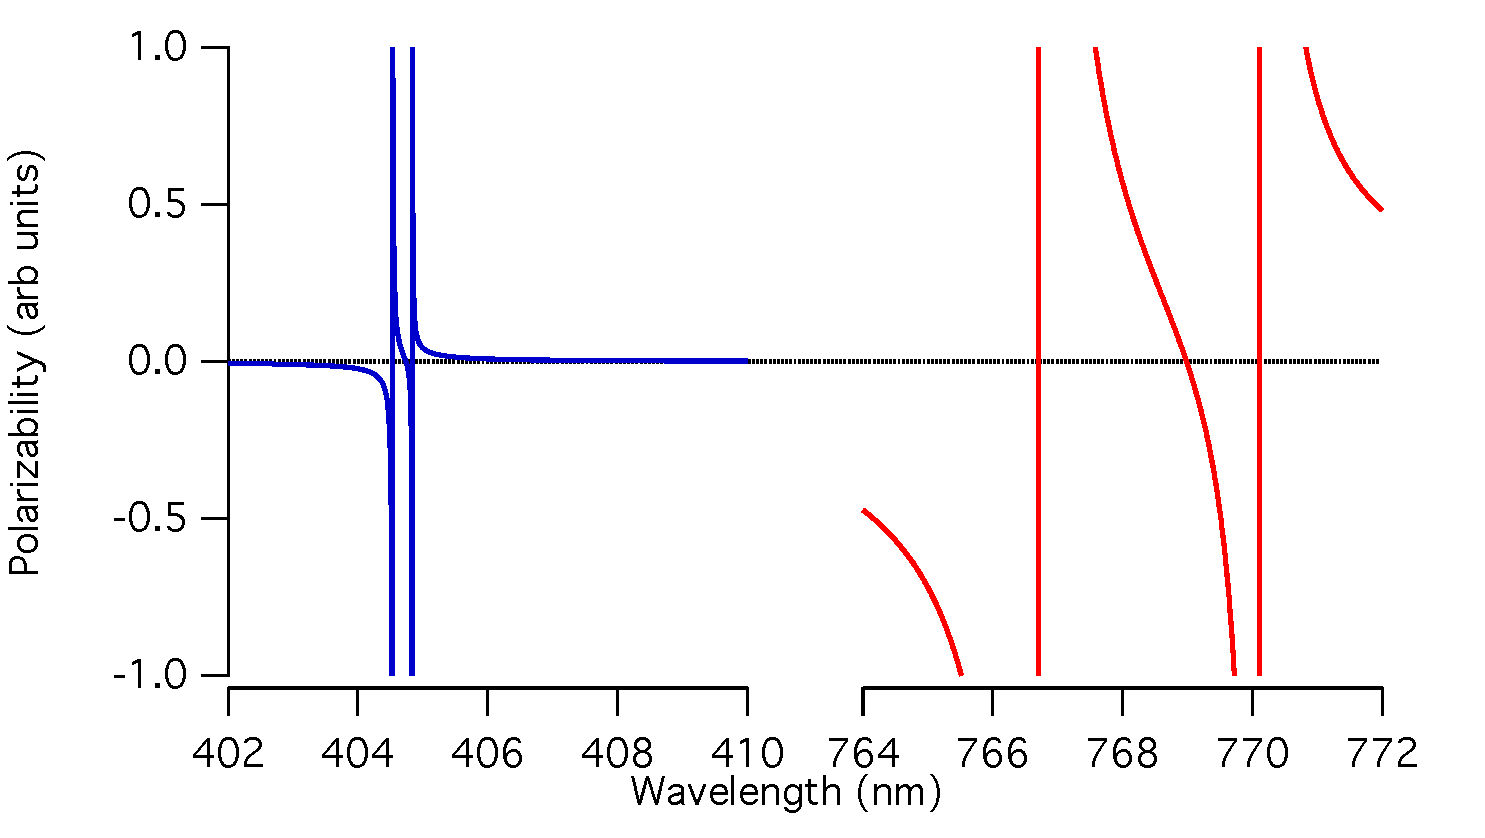
\includegraphics[width=.90\textwidth]{KredBlueMZW.pdf}
\caption{\label{KredBlueMZWfig}3 MZW in K}
\end{figure}

supplemental material?

contrast loss model? circular polarization discussion?

derivation of maximum slope?

ASE model?

NIST ASD grapher? make available at atomwave.org?

\subsection{Next-generation study?}
Hall-of-mirrors, bow-tie cavity, hole-in mirror. Figure from NSF proposal?
\begin{figure}
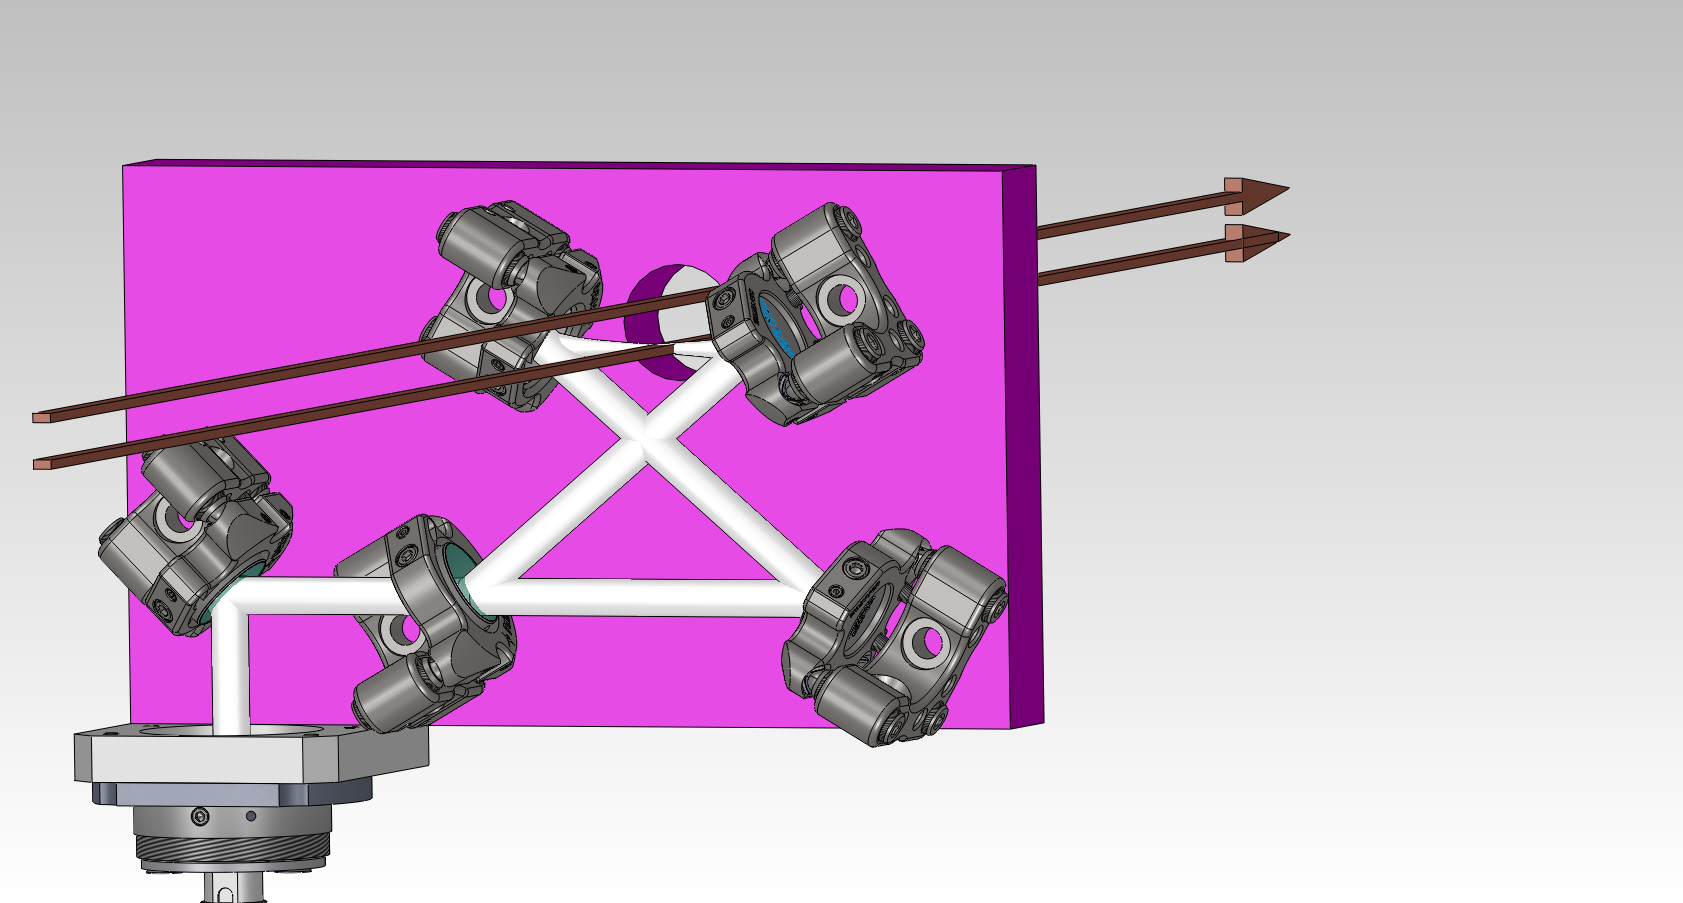
\includegraphics[width=.90\textwidth]{mzwCavityThruHole2.jpg}
\caption{\label{mzwCavityFig}MZW cavity figure}
\end{figure}

